\chapter{Radiation heat transfer}

\modinfo{Directory}{TemperatureRadiation}
\modinfo{Solvers}{\Idx{HeatSolve}}
\modinfo{Tools}{\Idx{ElmerGrid}, editor}
\modinfo{Dimensions}{2D, Axi-Symmetric}

\subsection*{Case definition}

At high temperature the radiation heat transfer between walls 
is often the dominating heat transfer mechanism. In this
tutorial we examine how radiation heat transfer between 
concentric cylinders is modeled. 


\subsection*{Solution Procedure}

The problem is a pure heat transfer problem that may be solved
with \texttt{HeatSolve}. The view and Gebharht factors 
associated with the radiation are solved as a first step 
in solving the equations. Thereafter the nonlinear heat equation is solved
until convergence is reached.

The computational mesh is done with \texttt{ElmerGrid} in directory \texttt{radiation} 
with the command 
\ttbegin
ElmerGrid 1 2 radiation
\ttend
The directory is given in the header of the command file
\ttbegin
Header
  Mesh DB "." "radiation"
End
\ttend
%
The only constant required is the Stefan-Boltzmann constant that gives the
relationship between temperature and radiation power
\ttbegin
Constants
  Stefan Boltzmann = 5.67e-8
End
\ttend
%
The geometry is axisymmetric and the case is solved in steady state.
As there is only one equation only 1 iteration for the system is required.
\ttbegin
Simulation
  Coordinate System = Axi Symmetric
  Simulation Type = Steady State
  Steady State Max Iterations = 1
  Output Intervals = 1
  Output File = "radiation.result"
  Post File = "radiation.vtu"
End
\ttend
% 
There are two bodies with the same equation but different properties.
\ttbegin
Body 1
  Equation = 1
  Body Force = 1
  Material = 1
  Initial Condition = 1
End

Body 2
  Equation = 1
  Material = 2
  Initial Condition = 1
End
\ttend
%
The nonlinear equation requires realistic initial conditions. Otherwise convergence
may not be obtained.
\ttbegin
Initial Condition 1
  Temperature = 250.0
End
\ttend
The body force is the heating power in units W/kg. 
\ttbegin
Body Force 1
  Heat Source = 10000
End
\ttend
The material properties differ only in heat conductivity. Heat capacity is not
actually needed since the case is not transient.
\ttbegin
Material 1
   Density = 1.0
   Heat Conductivity = 10.0
   Heat Capacity = 1.0
End

Material 2
   Density = 1.0
   Heat Conductivity = 1.0
   Heat Capacity = 1.0
End
\ttend
The heat equation is solved with an iterative procedure that requires some relaxation 
for better convergence. There are two different ways to discretize the radiation. 
There are two keywords defining when to switch to the true Newtonian iteration
which should give better convergence.
\ttbegin
Solver 1
  Equation = Heat Equation
  Stabilize = True
  Linear System Solver = Iterative
  Linear System Iterative Method = BiCGStab
  Linear System Convergence Tolerance = 1.0e-12
  Linear System Max Iterations = 500
  Linear System Preconditioning = ILU1
  Nonlinear System Newton After Iterations = 1
  Nonlinear System Newton After Tolerance = 1.0e-4
  Nonlinear System Max Iterations = 50
  NonLinear System Convergence Tolerance = 1.0e-8
  Steady State Convergence Tolerance = 1.0e-8
  Nonlinear System Relaxation Factor = 0.7
End
\ttend
The only solver is the heat equation.
\ttbegin
Equation 1
  Active Solvers = 1
End
\ttend
%
The radiation boundary conditions are set for two different boundaries. The first one
is for the internal object and the second one for the insulation. The normal direction
of the surfaces is important since a wrong direction may result to a badly set problem for
the view factor computation. Internal and external surfaces are very different.
The normal direction may be switched with the keyword \texttt{Radiation Target Body}.
A good sign of a properly set case is that the view factors add up to about one.
\ttbegin
Boundary Condition 1
   Target Boundaries = 1
   Heat Flux BC = True
   Radiation = Diffuse Gray
   Radiation Target Body = -1
   Emissivity = 0.6
End

Boundary Condition 2
   Target Boundaries = 2
   Heat Flux BC = True
   Radiation = Diffuse Gray
   Radiation Target Body = -1
   Emissivity = 0.1
End
\ttend
%
The third boundary condition is the Dirichtlet condition for the external boundary.
Dirichtlet conditions boost up the convergence even though the heat equation is basically
well defined also with external radiation conditions.
\ttbegin
Boundary Condition 3
   Target Boundaries = 3
   Temperature = 100.0
End
\ttend


\subsection*{Results}

For the current version of the case use Paraview (or some other
VTK based visualization tool) to view the results. 

\begin{figure}
\begin{center}
  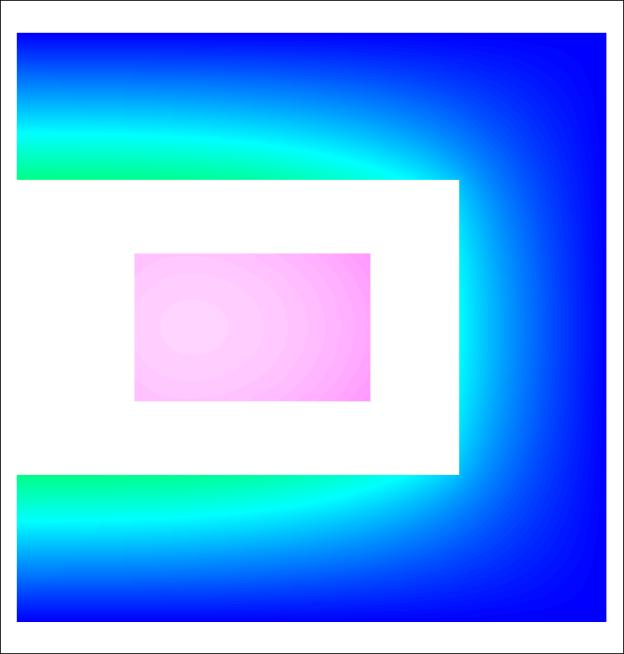
\includegraphics[height=0.6\textwidth]{radiation}
\end{center}
\caption{Temperature distribution in the radiation heat transfer
problem}
\label{fig:temp_rad1}
\end{figure}
 
With the given computational mesh the problem is solved in 
a few seconds. With 1,231 second order 9-noded
rectangular elements the maximum temperature is 565.7~K.
The corresponding results are shown
in Fig.~\ref{fig:temp_rad1}.

\hfill
